%% 
%% Libro en español
%% Pantilla Latex para estructura de un libro en español
%% Autor: Dario A. Palminio
%% LaTeX versión: 2.0
%% Sistema operativo: Ubuntu
%% Editor usado: LaTeXila 2.4.0
%% 

% Document pattern and general formatt
\documentclass[a4paper,11pt]{book}

% Imports
\usepackage[T1]{fontenc}
\usepackage[utf8]{inputenc} %% file charset=utf-8
\usepackage{lmodern}
\usepackage{graphicx}

% Image location
\graphicspath{ {images/} }

% Rename names to spanish language
\renewcommand{\contentsname}{Índice}
\renewcommand{\chaptername}{Capítulo}
\renewcommand{\bibname}{Bibliografía} % Bibliography in spanish
\renewcommand{\figurename}{Figura}

\begin{document}

% General structure
%%%%%%%%%%%%%%%%%%%%%%%%%%%%%%%%%%%%%%%%%%%%%%%%%%%%%%%%%%%%%\
%%%% Author & title page info

% Book's title and subtitle
\title{\Huge 
    \textbf{Ingeniería y Gestión de Proyectos con Scrum}  \\ 
    \huge 
    }

% Book's author
\author{Dario Palminio}

% Book's date
\date{2015} 

\maketitle


%% 

\tableofcontents
\newpage
\listoffigures
%%\newpage
%%\listoftables



\chapter{Introducción}

\section{Consideraciones iniciales}

\subsection{Definición}

Scrum es un marco de trabajo (framework) para construir y mantener productos complejos \cite{SBOK-2013} \cite{Scrum-Alliance-2015}. 
Scrum funciona como una implementación del ciclo de mejora continua de Deming (PDCA) y como una implementación de los principios ágiles y principios Scrum. Hay que tener en cuenta que Scrum no es exactamente un proceso íntegro, metodología completa o una técnica para construir productos; sino que, es un marco de trabajo dentro del cual se pueden emplear varias técnicas y procesos \cite{Agile-Atlas-2012}. 

\subsection{Sobre si es una Metodología}

Hay quienes consideran que Scrum no es una metodología, entre otras cosas porque no especifia exactamente el cómo se hacen las cosas, 
sino que dice el qué hacer. Sin embrargo, hay autores y guías que tratan a Scrum como metodología \cite{SBOK-2013}. De hecho en el informe original de Ken Schwaber se habla de metodología \cite{Ken-Schwaber-1995}. En consecuencia, se puede encontrar en numerosa bibliografía que el marco de trabajo Scrum puede ser denominado Metodología de Desarrollo Scrum o Metodología de Gestión de Proyectos Scrum. 
En el primer caso puede deberse a que se puede considerar una metodología como un proceso de desarrollo iterativo e incremental de productos \cite{Ken-Schwaber-1995}. Y en el segundo caso porque se puede considerar que es una alternativa a la gestión clásica de proyectos propuesta por metodologías como la Metodología de Gestión de Proyectos PMI. En este último sentido podemos recordar la definición original de Ken Schwaber: "Scrum es una metodología de gestión, mejora y mantenimiento de un sistema existente o prototipo de producción" \cite{Ken-Schwaber-1995}.
 
Por otro lado, considerando que Scrum define roles, artefactos, actividades, flujo del ciclo de actividades Scrum \cite{Agile-Atlas-2012}, reglas y algunas sugerencias de implementación como, además, al definir el flujo del ciclo de Scrum o flujo de trabajo define parcialmente un cómo, en el cual incluye una secuencia básica de cosas a hacer; por eso, y sin ser puristas, se puede considerar como una forma de metodología de trabajo y de gestión. O sea que puede funcionar como una metodología a alto nivel o plataforma de trabajo sobre la cual pueden funcionar otras metodologías, más específicas de producción y desarrollo, y otras técnicas y procesos. Por este motivo, 
Scrum puede ser adaptado a diversas empresas y organizaciones que trabajen con metodologías diferentes pero compatibles con los 
lineamientos de Scrum (sus valores y principios) y del Movimiento Ágil (filosofía ágil). Se puede usar Scrum y a su vez utilizar técnicas de otras metodologías para implementar sus actividades y sugerencias. O sea que cuando se usa Scrum se hace una aproximación empleando diversas técnicas y, posiblemente, otras metodologías.

\subsection{Ámbito de aplicación}

Relacionado a su ámbito de aplicación se pude decir que Scrum no es un marco de trabajo orientado a implementarse en cualquier dominio y contexto. Scrum está pensado para proyectos bajo "dominios complejos" [Snowden 2007] donde existe un grado alto de incertidumbre y baja predictibilidad (ver figura \ref{fig:MarcoCynefinModel}). O sea que es útil en ámbitos con requisitos inciertos y riesgos técnicos altos. Nos permite encontrar prácticas emergentes en dominios complejos, como por ejemplo en la gestión de proyectos de innovación \cite{Martin-Alaimo-2014}. Está orientado a contextos que necesitan niveles altos de creatividad, innovación, interaccion y comunicación. Por este motivo, es bastante empleado en la industria de software, ya que en la misma existen contextos específicos de alta complejidad e incertidumbre con necesidad de creatividad e innovación. Pero también se utiliza en otras industrias con dominios de problemas de complejidad semejante. Por ejemplo ha sido empleado en: educación, organizaciones de campañas publicitarias, industria de productos de innovación, empresas de editoriales de libros, etcétera.

\begin{figure}[h]
  \centering
  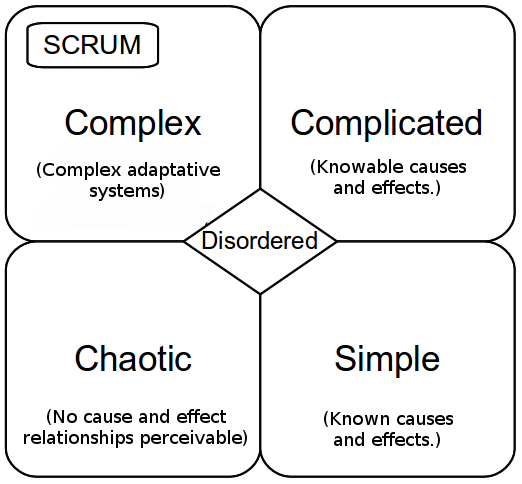
\includegraphics[width=0.50\textwidth]{MarcoCynefinModel}
  \caption{Modelo de dominios de Marco Cynefin}
  \centering
  \label{fig:MarcoCynefinModel} %\ref{fig:MarcoCynefinModel}
\end{figure}

\subsection{Visión general}

En esta metodología se definen los principios y valores a seguir, los roles, relaciones y respnsabilidades, los artefactos o entidades manejadas en el proceso de trabajo, un conjunto de reuniones o actividades en un flujo de trabajo como resume la imagen de la figura \ref{fig:ScrumMapMind}.

\begin{figure}[h]
  \centering
  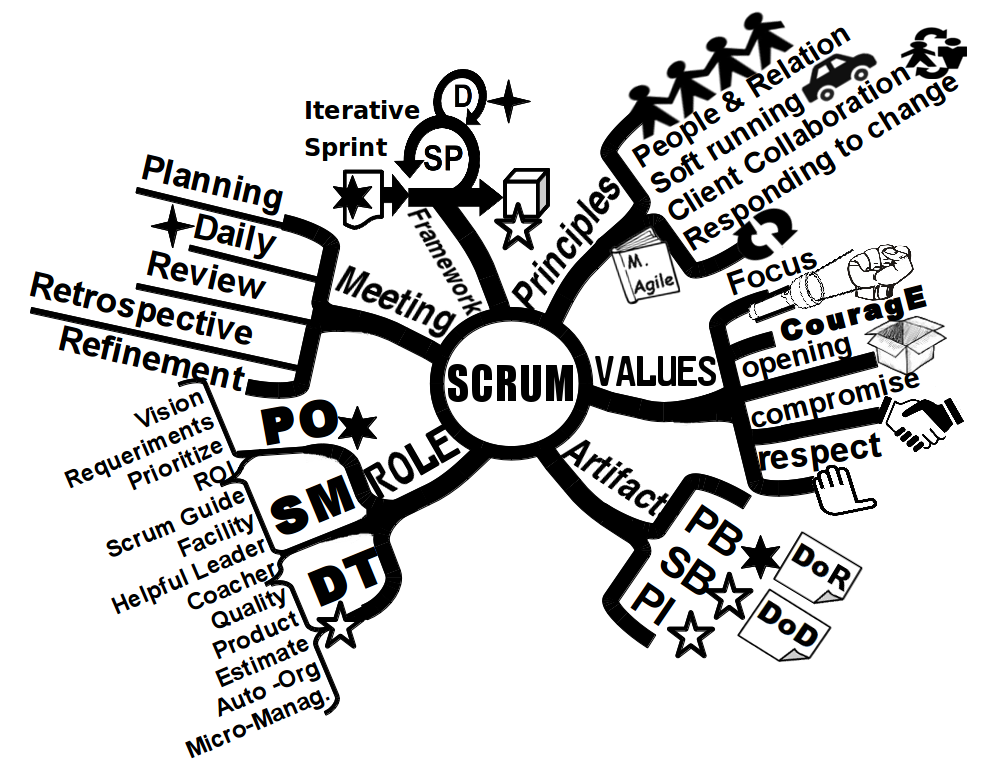
\includegraphics[width=0.99\textwidth]{ScrumMapMind}
  \caption{Mapa mental sobre Scrum}
  \centering
  \label{fig:ScrumMapMind} %\ref{fig:ScrumMapMind}
\end{figure}

En los siguientes capítulos se explicarán los diferentes aspectos y características de la propuesta de este marco de trabajo con lo que 
al final del libro el mapa mental de la figura \ref{fig:ScrumMapMind} quedará explicado y será fácilmente entendible. 

\chapter{Principios}

% Chapter about Scrum System core

\chapter{Núcleo del Sistema Scrum}

Scrum es un sistema compuesto por la filosofía Scrum (SCRUM Philosophy), como parte del sistema cultural, y tres conjuntos de componentes interrelacionados que forman el Núcleo del Sistema Scrum (ver figura \ref{fig:ScrumSystemCore}). Los tres conjuntos de componentes son: roles, actividades y artefactos. Los roles conforman un sistema de roles que determina las responsabilidades de los actores integrantes, sus relaciones recíprocas, sus restricciones y la relación con los demás componentes. Las actividades conforman la parte principal del sistema de procesos Scrum (Proceso Scrum) que determina las relaciones de organización entre actividades, roles y artefactos. Y los artefactos conforman el conjunto de almacenes o componentes de trabajo. Todo el sistema busca asegurar una cadencia de trabajo que consta de una regularidad basada en iteraciones de tiempo fijo y ceremonias o actividades regulares que permiten la repetibilidad rítmica (predictibilidad del flujo de trabajo) bajo un grado de prestancia.

A continuación se describirán estos componentes y sus relaciones.

\begin{figure}[h]
  \centering
  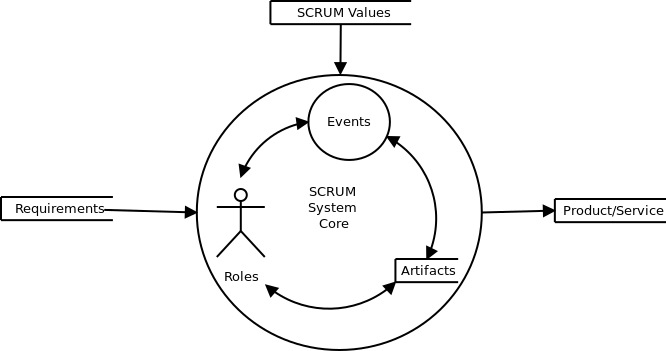
\includegraphics[width=0.99\textwidth]{ScrumSystemCore}
  \caption{Diagrama del Núcleo del Sistema Scrum}
  \centering
  \label{fig:ScrumSystemCore} %\ref{fig:ScrumSystemCore}
\end{figure}


\section{Estructura del Sistema Scrum}

Scrum está pensado como un sistema de trabajo para equipos con tres roles principales: el Product Owner, el Scrum Master y el Development Team. 

Cuando los integrantes del sistema Scrum ejercen los roles mencionados en un flujo de trabajo o proceso Scrum, trabajan sobre tres artefactos esenciales: el Product Backlog (lo que queda por hacer), el Sprint Backlog (lo que se va a hacer) y el Incremento de Producto (lo que logramos hacer). Estos artefactos son tratados en un flujo de trabajo en el cual se construyen productos en forma incremental, en una serie de ciclos cortos de tiempo llamados Sprints. 

En cada ciclo Sprint del flujo de trabajo se practican seis actividades Scrum: refinamiento de producto, planificación, reunión diaria o Daily, desarrollo, revisión de producto y retrospectiva. La actividad de refinamiento de producto (Refinement) no suele tener un nombre unificado; pues, se la suele llamar "Backlog Grooming"\footnote{No se aconseja usar el término Grooming debido a que según el diccionario Oxford English Dictionary tiene connotaciones sexuales.} (aunque no se aconseja usar la palabra grooming), Manteniemiento de Backlog o Refinamiento (Refinement). Salvo el desarrollo, las actividades se consideran reuniones o ceremonias Scrum. El desarrollo no es una reunión Scrum ya que constituye la actividad de producción del producto o servicio. O sea que es donde se produce el incremento de producto.

\section{Sistema de Roles}

El Sistema de Roles (ver figura \ref{fig:ScrumRolesSystem}), en el núcleo de Scrum, es el conjunto de roles y relaciones parte del sistema Scrum. Como se mencionó anteriormente hay tres roles principales: el Product Owner o dueño del producto, el Scrum Master o facilitador y el Equipo de Desarrollo o Equipo a secas (Scrum Development Team, Miembros del Equipo de Desarrollo o Desarrolladores Scrum). También hay roles secundarios como el de Stakeholder, Vendedores y Cuerpo de Asesoramiento de Scrum. El rol Stakeholder es el más importante de los roles secundarios e incluye a los clientes, usuarios y patrocinadores\footnote{\cite{SBOK-2013}}.

Hay que tener en cuenta que Scrum contempla solo estos tres roles principales como núcleo en el equipo Scrum y cuando se implementa en forma ortodoxa son los únicos roles permitidos. En el caso del Equipo de Desarrollo, cada integrante puede tener diferentes perfiles, características o roles especializados, pero bajo este marco sólo tienen el rol de Desarrollador. Cuando Scrum se integra con otras metodologías o esquemas de roles los desarrolladores pueden cumplir otros roles que funcionan como sub-roles.

\begin{figure}[h]
  \centering
  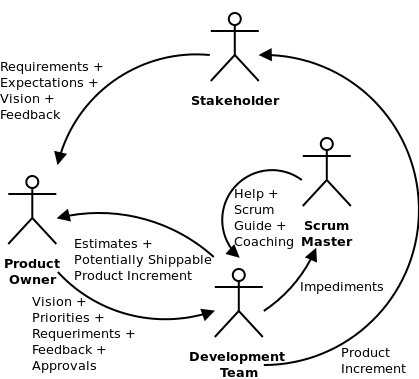
\includegraphics[width=0.80\textwidth]{ScrumRolesSystem}
  \caption{Diagrama del Sistema de Roles Scrum}
  \centering
  \label{fig:ScrumRolesSystem} %\ref{fig:ScrumRolesSystem}
\end{figure}

A continuación se listan los diferentes roles principales:

\subsection{Equipo de Desarrollo}

El Equipo de Desarrollo es parte del Equipo Scrum y son los responsables de construir, o sea desarrollar el producto.
 
Para el cumplimiento del rol Equipo de Desarrollo o desarrollador se deben tener en cuenta las siguientes afirmaciones:

\begin{itemize}
\item Crea y gestiona el desarrollo de software comprometiéndose a fechas de entregas estimadas.
\item Es responsable de la calidad técnica del producto.
\item Debe buscar su desarrollo profesional para lograr excelencia técnica. Para ello debe, además, mantener el foco en el aprendizaje, la innovación y el mantenimiento de una actitud de mejora contínua.
\item Debe evitar trabajar en múltiples proyectos teniendo asignación cien por ciento en el proyecto.
\item Debe priorizar y promover la comunicación cara a cara.
\item Provee estimaciones de ítems de trabajo.
\item Es responsable de gestionar su propio trabajo durante el Sprint.
\item Buscar encontrar una cadencia sostenible para la entrega de incrementos potencialmente entregable de productos.
\item No debe esperar a que le asignen tareas ya que debe seguir la forma "pull" de asignación que consiste en tomar tareas por sí mismo o por consenso de todo el equipo.
\item Monitorea el progreso y el éxito con el resto de los roles del Scrum Team.
\item No debe ocultar impedimentos ni información.
\item No debe hacer tareas de otro rol Scrum. En el caso de una implementación ortodoxa no tiene otro rol que el de desarrollador.
\item Debe procurar ser multidisciplinario aprendiendo del conocimientos de los compañeros, aplicando sus habilidades en diferentes tipos de tareas y no especializándose en una sola cosa donde se trabaja en forma estanco (cerrada y hermética).
\item Debe procurar la estabilidad del equipo y su cadencia.
\end{itemize}

\subsection{Product Owner}

El "Product Owner" cumple la función de dueño del producto en el proyecto y es el responsable del negocio. O sea que, es el "Responsable del Producto" o Servicio, quien vela por que el equipo tenga una visión clara y una estrategia, de qué es lo que se va a hacer, para la creación de ese producto o servicio.

Para el cumplimiento del rol Product Owner se deben tener en cuenta las siguientes afirmaciones:

\begin{itemize}
\item Debe colaborar con el Scrum Master y con el Equipo de Desarrollo.
\item Es quien determina el mejor producto a conseguir.
\item Es quien provee las "hipótesis requerimientos"\footnote{Bajo el marco Scrum los requerimientos inicialmente constan de hipótesis a ser evaluadas. Son hipótesis porque son dinámicas, no son requerimientos finales sino que son deseos del cliente a ser refinados hasta convertirse en verdaderamente requerimientos.}, por lo que es responsable de entenderlas, escribirlas y transmitirlas en forma eficaz.
\item Es dueño y responsable por el artefacto Product Backlog.
\item Es responsable de formar una visión, comunicarla y promoverla.
\item Es responsable del retorno de la inversión ROI y de los resultados empresariales, evaluando continuamente el impacto en el negocio.
\item Es recomendable que esté asignado a un solo Scrum Team con un porcentaje de asignación del 70 al 80 por ciento.
\item Asegura la Colaboración efectiva y la participación de los Stakeholders en el proyecto, administrando sus expectativas y manteniendo una comunicación regular con ellos.
\item Monitorea el progreso y el éxito con el resto de los roles del Scrum Team.
\item No estima ni provee estimaciones.
\item No gestiona el presupuesto de todo el proyecto pero puede gestionar el presupuesto del equipo.
\item No es jefe ni gerente de proyecto.
\end{itemize}

\subsection{Scrum Master}

El Scrum Master es un "Facilitador" y "Coach del Equipo", que es guardián del marco de trabajo Scrum y responsable de mejorar el flujo de valor hacia el cliente. Que sea guardián del marco de trabajo significa que es quien debe asegurar que se siga el sistema Scrum, concientizar sobre la filosofía seguida bajo el mismo, capacitar y entrenar al equipo de desarrollo y facilitar la resolución de impedimentos relacionados a la implementación de Scrum.

Para el cumplimiento del rol Scrum Master se deben tener en cuenta las siguientes afirmaciones:

\begin{itemize}
\item Es el responsable de que se siga Scrum. Brinda apoyo a las prácticas de Scrum.
\item Necesita desempeñar su rol con coraje.
\item Debe gestionar los riesgos y problemas junto con los demás roles.
\item Debe buscar remover obstáculos e impedimentos.
\item Es responsable de buscar lograr la mejora continua del proceso o sistema de trabajo.
\item Busca conseguir que se haga el trabajo.
\item La mejor manera de cumplir el rol es estar tiempo completo en este rol (asignación 100 por ciento).
\item Sirve de embajador del equipo ante la organización, obrando en ocasiones como mensajero, representante o interfaz.
\item Debe ser guardián del equipo protegiéndolo de perturbaciones externas negativas.
\item Monitorea el progreso y el éxito con el resto de los roles del Scrum Team.
\item Ayuda al Equipo a encontrar una cadencia sostenible para la entrega de incrementos potencialmente entregable de productos. 
\item Busca lograr un entorno seguro y de apoyo que genere confianza y respeto mutuo. Ayuda a lidiar con los conflictos personales.
\item Busca establecer acuerdos claros y que se cumpla lo pactado.
\item Colabora con el proceso de aprendizaje del equipo.
\item Considera diferentes formas de trabajar con el equipo Scrum buscando aplicar las más adecuadas según el contexto.
\item Busca comprender la esencia de la comunicación en los diálogos del equipo Scrum y ayudar a concretar sus acciones y su entendimiento.
\item La presencia en la Daily Scrum no es obligatoria, pero es aconsejable que esté para facilitarla y moderarla cuando sea necesario.
\item No debe estimar junto al Equipo de Desarrollo ni hacer tareas de otro rol como, por ejemplo, desarrollar (programar, probar, etc.).
\item No es jefe, no es gerente de proyecto, no debe gestionar al Equipo de Desarrollo y no es responsable por la planificación del proyecto.
\item No asigna tareas, sino que procura que el equipo se las auto-asigne o las tome por voluntad propia y auto-organización.
\end{itemize}


\section{Proceso Scrum}

En el proceso Scrum o sistema de flujo de actividades Scrum (ver figura \ref{fig:ScrumFlow}) los miembros del equipo Scrum colaboran para crear una serie de Incrementos de Producto durante iteraciones de intervalos fijos de tiempo denominados Sprints. En cada iteración Sprint, se comienza por una Planificación del Sprint para producir un Backlog del Sprint a partir del Backlog de Producto, es decir un plan para el Sprint. El equipo se auto-organiza para realizar el Desarrollo, mediante reuniones Diarias de Scrum para coordinar y asegurarse de estar produciendo el mejor Incremento de Producto posible en el proceso de desarrollo del producto o servicio. Cada incremento satisface el criterio de aceptación del Product Owner y la Definición de Hecho o "Definition of Done" compartida por el equipo para satisfacer el criterio de tarea terminada. Junto al proceso de desarrollo se hace también un Refinamiento del Backlog ("Refinement") para prepararse para la reunión de planificación del próximo Sprint. Finalizando cada ciclo se termina el Sprint con una reunión de Revisión del Sprint y luego una reunión Retrospectiva del Sprint, revisando el producto y su proceso con una perspectiva crítica y de mejora contínua. 

\begin{figure}[h]
  \centering
  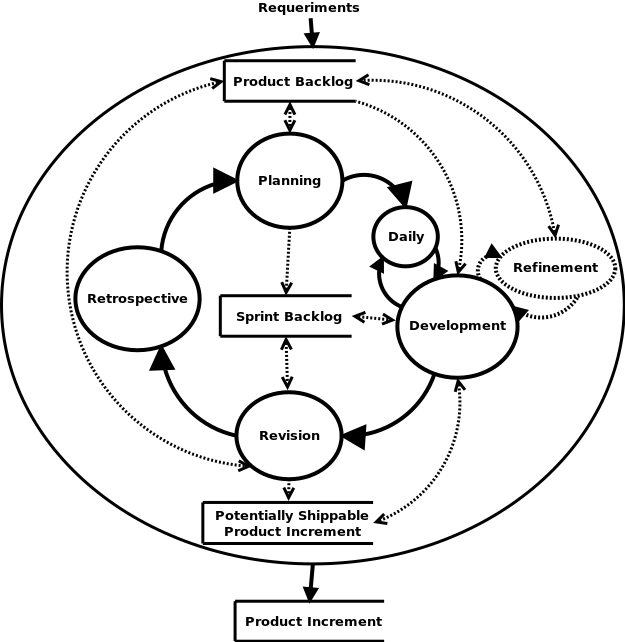
\includegraphics[width=0.99\textwidth]{ScrumFlow}
  \caption{Diagrama de Flujo de Datos del Proceso Scrum}
  \centering
  \label{fig:ScrumFlow} %\ref{fig:ScrumFlow}
\end{figure}

\subsection{Reuniones principales}

\begin{itemize}

\item \textbf{Planificación:} es una actividad o una conversación de duración fija al principio de cada Sprint para decidir sobre lo que se terminará y se demostrará en la revisión.

Esta reunión se divide generalmente en tres partes principales: una primera parte es estratégica relacionada al "qué", una segunda parte táctica relacionada al "cómo" y una tercera relacionada al acuerdo de cierre. 

\begin{itemize}

\item \textbf{Planificación relacionada al "Qué":} La primera parte se propone responder a: ¿Qué trabajo será realizado? En esta parte se desarrolla la definición de lo que se necesita hacer, de cuáles hipótesis del Cliente se desean desarrollar. En este proceso se crean los ítems de Product Backlog o PBIs y los Criterio de Aceptación. Los PBIs son generalmente escritos por el Product Owner y están diseñados para asegurar que las hipótesis de requisitos del Cliente estén claramente representados y puedan ser plenamente comprendidos por todos los Stakeholders y los desarrolladores del Equipo.
En la dinámica de la reunión el Product Owner cuenta cuáles son los PBIs disponibles, que pasan el criterio de completitud o DoR (una definición de terminado), para ser desarrollados en el Sprint y los explica para que sean comprendidos por el Equipo. Mientras sucede esto los integrantes del Equipo hacen todas las preguntas que consideren necesarias para comprender los detalles de lo que se desea realizar y puedan, así, entregar una estimación del trabajo a comprometer. Luego de estimar se procede a una negociación entre el Product Owner y el Equipo de cuáles son los PBIs que el Equipo se compromete a desarrollar para transformar en un incremento de producto potencialmente entregable. En este proceso el Scrum Master se encarga de facilitar la ceremonia, moderar y tratar de asegurar de que todos los Stakeholder del proyecto que sean necesarios para para aclarar detalles estén presentes o sean contactados para hacer las respectivas aclaraciones.
El resultado de este proceso es un conjunto de PBIs estimados y comprometidos inicialmente para ser trabajados en el Sprint.

\item \textbf{Planificación relacionada al "Cómo":} En la segunda parte de la planificación se propone responder a: ¿Cómo será realizado el trabajo? Esta parte es táctica y por lo tanto más técnica por lo que no es necesaria la presencia del Product Owner, pero debe estar disponible para contestar preguntas y clarificar dudas surgidas sobre la marcha. En esta reunión el Equipo discute cómo implementará los PBIs, diseñando inicialmente, en forma general y abstracta (acuerdo de alto nivel), las soluciones y definiendo tareas implicadas. 

\item \textbf{Cierre de planificación como "Acuerdo":} Cuando termina la reunión relacionada al "Cómo", el Equipo debe negociar y comprometer finalmente el alcance del Sprint formando un acuerdo de compromiso con el Product Owner. El resultado de este proceso es un conjunto de PBIs que forman el alcance del Sprint, o sea el Sprint Backlog, el objetivo del Sprint y una visión de diseño o arquitectura a alto nivel de lo que se desea implementar junto con un conjunto de tareas planificadas para el Sprint.

\end{itemize}

\item \textbf{Scrum Diario:} es una actividad o una reunión diaria obligatoria del Equipo Scrum, en el lugar de trabajo, con una duración fija, que sirve para coordinación y organización mediante una retroalimentación del estado de actividades de cada integrante del Equipo. Permite identificar impedimentos bloqueantes, actualizar artefactos, revisar el Sprint Backlog, ayudar a disminuir riesgos e identificar personas que pueden servir de ayuda a determinadas tareas. En esta reunión los miembros del equipo se reúnen, de pie, para informar de sus progresos en el Sprint y planificar las actividades del día. Para ello proporcionan respuestas a tres preguntas:

\begin{itemize}
\item{¿Qué hice ayer?}
\item{¿Qué voy a hacer hoy?}
\item{Si tengo obstáculos: ¿Qué impedimentos tengo?}
\end{itemize}

Es obligatorio que el Equipo asista a esta reunión y es aconsejable que esté el Scrum Master para facilitarla y servir de moderador. El PO puede asistir también para seguir el avance del trabajo durante la iteración, pero puede no participa activamente, sino como oyente. Sin embargo, si se quiere lograr un mejor trabajo de equipo y mayor integración con el PO, es aconsejable que siga la dinámica al igual que el Equipo.

\item \textbf{Refinamiento:} es una actividad o reunión para refinar la lista de PBIs o Product Backlog que consiste en trabajar sobre las hipótesis de requerimientos, definirlas y añadirles detalles, granularizarlas, estimarlas y priorizarlas. Es un proceso continuo que hace el Product Owner, pero formalmente como reunión se desarrolla con participación del Equipo en colaboración para examinar y revisar los elementos del Product Backlog. En esta reunión la responsabilidad recae en el Product Owner y el Equipo solo colabora.

En la reunión que se hace con el equipo se desarrollan las siguientes actividades:
  \begin{itemize}
  \item{El PO presenta los próximos ítems de backlog al equipo.}
  \item{Se conversa grupalmente aspectos sobre ítems de backlog: }
    \begin{itemize}
    \item{Conversación, entendimiento y ajuste.}
    \item{Búsqueda de posibilidad de granularización.}
    \item{Identificación de dependencias.}
    \item{Detección de riesgos que pueden hacer que esas historias no se completen e identificación de actividades a realizar para mitigarlos.}
    \end{itemize}
  \item{Estimación.}
  \item{Priorización.}
  \end{itemize}

\item \textbf{Revisión:} es una actividad o una conversación de duración fija al final de cada Sprint para dar retroalimentación sobre el avance del producto. En esta reunión se evalúa el incremento funcional potencialmente entregable construido por el Equipo en el proceso de desarrollo. Para lograr hacer esto el Equipo de Desarrollo junto al Product Owner y los Stakeholder involucrados, revisan los resultados funcionales y operativos (producto utilizable) del Sprint. El objetivo es recibir una retroalimentación de lo construido y aprobar o rechazar los PBIs que pasaron la DoD y son potencialmente entregables, para lo que los Stakeholder prueban el producto construido y proveen su feedback. En este proceso pueden haber cambios o nuevas hipótesis de requisitos que surjan para agregarse en el Product Backlog.

\item \textbf{Retrospectiva:} es una actividad o una conversación de duración fija al final de cada Sprint para que el Equipo reflexione y busque mejoras procedimentales. En esta reunión se intentan responder tres preguntas relacionadas al "proceso": ¿qué se hizo mal?; ¿qué se hizo bien? y ¿que se puede mejorar?
De esta reunión deberían quedar lecciones aprendidas y un listado de acciones a tomar para mejorar la forma de trabajar. Las acciones a tomar deben ser desarrolladas en el siguiente Sprint y analizadas en la retrospectiva del mismo.

\end{itemize}

\section{Flujo de artefactos}

Los artefactos ítems de trabajo fluyen desde que se definen en el Backlog de Producto hasta que se transforman en incremento de producto. Los ítems de trabajo son items de valor para el cliente que comienzan su nacimiento como ítems de backlog o PBIs del Backlog de Producto. Debido a que el dueño del Backlog de Producto es el Product Owner, es él quien crea los PBIs, ya sea por trabajo individual o con la colaboración del Equipo de Desarrollo. Los PBIs son requerimientos que puede escribirse de diferente manera. Es común escribir los PBIs en forma de Historias de Usuario \cite{Cohn-2004}, pero no es un requisito de Scrum. Estos PBIs son refinados por la actividad de Refinamiento de Backlog hecha por el Product Owner y el Equipo de Desarrollo mientras se practica el desarrollo de un Sprint y son priorizados por el ProductOwner. El la la reunión de planificación "Planning" se toman PBIs que cumplan el criterio de aceptación o "Definition of Ready" (2 "Selection") para ser incluidos en el "Sprint Backlog" y el Equipo de Desarrollo pueda trabajar en ellos en el Sprint. A medida que el Equipo de Desarrollo termina un ítem "Sprint Backlog" cumpliendo el criterio de aceptación "Definition of Done" (3 "increment") se genera un Incremento de Producto candidato potencialmente entregable (Potentially Shippable Product Increment). Luego en la Revisión se acepta el Incremento de Producto candidato pasando a ser efectivamente un Incremento de Producto listo para ser entregado o desplegado, para "Release" (4 "releasing"). En caso de no ser aprobado (5 "Rejection") pasa nuevamente al Product Backlog para ser tenido en cuenta en el próximo Sprint. Los ítems de "Sprint Backlog" que no se lograron terminar también vuelven (6 "comeback") al "Product Backlog". Esto ocurre formalmente en la revisión \cite{Martin-Alaimo-2014}.

\begin{figure}[h]
  \centering
  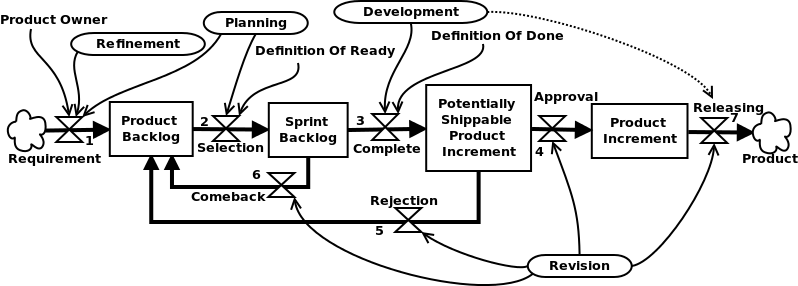
\includegraphics[width=0.99\textwidth]{ScrumArtifactsStockFlow}
  \caption{Diagrama de Flujo de Stock de artefactos Scrum}
  \centering
  \label{fig:ScrumArtifactsStockFlow} %\ref{fig:ScrumArtifactsStockFlow}
\end{figure}

\subsection{Definición de preparado}

La definición de preparado, "Definition of Ready" o DoR es una Definición de Terminado particular que se corresponde con las condiciones para que un PBI pueda pasar a formar parte de un Sprint Backlog. Si un PBI no cumple con su DoR no puede ser tomado en una planificación para ser ítem de trabajo del Sprint planeado, ya que es un ítem que no está suficientemente preparado para ser comprometido. O sea que, la definición de preparado permite entonces tener un punto de acuerdo entre el Product Owner y el Equipo, permitiendo conocer cuándo una historia de usuario está realmente lista para evaluar su factibilidad de desarrollo en una reunión de planeamiento y ser llevada a un Sprint.

Un ejemplo de DoR puede ser el que sigue:

\begin{enumerate}
\item{Historia de usuario definida.}
\item{Cumple el criterio INVEST (INVEST es tratado posteriormente).}
\item{Hay un contexto de negocio claro.}
\item{Criterios de aceptación definidos, claros y comprobables.}
\item{Identificación de dependencias con otras historias de usuario.}
\item{Hay una idea clara de cómo se puede demostrar la historia en una review.}
\item{El equipo tiene el conocimiento para analizarla.}
\end{enumerate}

\subsection{Definición de Terminado}

Los ítems de artefactos fluyen por sus diferentes estados (o Stock en el flujo de Stock) a medida que cumplen con determinadas condiciones de cambio de estado. A estas condiciones que deben cumplir para cambiar de estado se las llama definición de terminado y funcionan como válvulas para que los ítems pasen de un Stock a otro Stock. Por ejemplo para que un ítem pase del Stock de Sprint Backlog a Incremento de Producto Potencialmente Entregable debe cumplir una definición de terminado, "Definition of Done" o DoD. Normalmente se suele considerar que el DoD es una lista de actividades que cada elemento de trabajo debe completar para poder ser considerado potencialmente entregable para un cliente dado y conforma un "entendimiento compartido de lo que significa que el trabajo esté completado"\footnote{\cite{Ken-Jeff-2013}}.

\section{Reglas y Consideraciones}

Además se establecen alguna consideraciones relacionadas a tiempos y tamaños. Se aconseja un tamaño de equipo de desarrollo mayor a 4 miembros y menor a diez (7 +- 2), o sea entre cinco y nueve. Por debajo de este número mínimo se tiene un equipo pobre que puede brindar un producto pobre y por sobre ese número máximo se aumenta la complejidad de gestión y coordinación del equipo disminuyendo el funcionamiento apropiado tras la metodología planteada. También se recomienda una duración de Sprint no mayor a un mes \cite{Ken-Jeff-2013}. La Reunión de Planificación de Sprint debería tener un máximo de duración de ocho horas para un Sprint de un mes. El Scrum Diario o "daily" es una reunión con un bloque de tiempo de 15 minutos para que el Equipo de Desarrollo sincronice sus actividades y cree un plan para el día. Por ejemplo, una daily de mayor de 15 minutos se puede considerar larga y en 15 minutos es complicado que mas de 15 personas puedan exponer lo que hicieron, lo que harán y si tienen bloqueos. Por eso se aconseja como máximo nueve personas en el equiopo de desarrollo. En lo que concierne a la Revisión, el tiempo estipulado es de cuatro horas para Sprints de un mes o dos horas para uno de una quincena. La reunión de Retrospectiva  debería estar restringida a un bloque de tiempo de tres horas para Sprints de un mes o  a una hora y media para los de una quincena. Las reuniones de Planificación, Revisión y Retrospectiva deberían ser proporcionales a la duración del Sprint.

\chapter{Escalamiento}

Scrum es aconsejable para ser óptimo en equipos chicos y proyectos pequeños, con agrupación de personas de múltiples disciplinas en un solo equipo para maximizar el ancho de banda de las comunicaciones, la visibilidad y la confianza. Esto sucede porque cuando los equipos son grandes aumenta el acoplamiento de individuos complejizando las comunicaciones y dificultando la coordinación y el buen desarrollo de las reuniones Scrum. Además se desprende del principio o Ley de Brooks, que dice que cuando se agregan personas a un proyecto o equipo aumentan los canales de comunicación pudiendo generar sobrecarga de comunicación. Por este motivo y desde un punto de vista purista, cuando se quiere implementar Scrum en proyectos grandes que requieren muchas personas, en su forma ortodoxa, no es recomendable. Pero se han encontrado maneras organizativas para aplicar Scrum en estos casos, como así también en grandes organizaciones. A esto se llama "Scaling Scrum" o Escalamiento de Scrum.

En "Scaling Scrum" los desafíos más importantes son: manejar las dependencias e integrar el trabajo en todos los niveles. En general Scrum se escala mediante reproducción de equipos con configuraciones adecuadas y la cohesión y acoplamiento mediante algún sistema de integración ágil, como el uso de "Scrum de Scrum", equipos de Product Owners, equipo de integración, etcétera. Hay varios casos que se pueden investigar, como por ejemplo las implementaciones de: Google, Spotify, Adobe, Nexus, etc.

\section{Formación de equipos}

Cuando migramos desde una organización tradicional, de management 1.0, a una ágil, tal vez uno de los desafíos más relevantes y difíciles es el de organizar equipos. ¿Cómo juntamos a las personas apropiadas en forma sostenida en el tiempo? Para que un equipo sea uno, debe tener un propósito claro y distinguible de otro de la compañía. Y, en consecuencia, debería tener todas las habilidades y competencias necesarias para cumplir el propósito de forma sostenida en el tiempo. Cuando ya tenemos equipos Scrum formados, tal vez la tarea sea más fácil. Pues, en "Scaling Scrum" los equipos funcionan como células que, a medida que la organización se expande, se clonan sus estructuras como en reproducción celular. Las estructuras de las células dependen del problema que se quiere resolver en cada caso y según los nuevos propósitos que surjan. 

De esta idea se desprende la pregunta de ¿qué propósito damos a cada equipo? o ¿cómo estructuramos a los equipos según qué propósitos? Una manera de hacerlo, pensando en productos y en el sector de producción de la compañía, es tomando una unidad de negocio o producto y ver si su alcance o tamaño es suficiente para un equipo o para varios. Si es para varios, una forma es analizar la jornada o flujo de experiencia del producto, determinar los KPIs involucrados y desglosar en subproductos con sus KPIs asociados. Así cada equipo puede ser responsable de un subproducto y de impactar según los KPIs identificados. Esta es una manera de hacerlo de arriba hacia abajo y orientados a producto. Luego, otra pregunta que surge es: ¿cómo los estructuramos? Bien, si el equipo es de producción como el desarrollo de software de productos, con trabajo planificable y divisible en lotes, Scrum viene como anillo al dedo. O sea que necesitamos a un SM y un PO en el equipo. Un equipo Scrum puede estar formado por diferentes roles, tales como: UX, SM, PO, BA, QA, FE Dev, BE Dev, etcétera. Por ejemplo, un equipo puede estar formado por: PO, SM, UX, 3 FE Dev y 3 BE Dev; otra estructura puede ser: PO, SM, BA, QA, 2 FE Dev y 2 BE Dev. O sea que podemos tener una infinidad de configuraciones. ¿Cuál puede ser la apropiada? No solo depende del propósito, sino de cómo desarrollaremos ese propósito o cuán autónomos somos en relación a él. En esta vía tenemos tres lineamientos básicos de configuración: equipos Scrum de características, equipos Scrum de componentes o uno mixto. Y cada una de estas modalidades pueden tener diversas configuraciones de roles.

\subsection{Equipos de características}

Abordar el problema de proyectos grandes con "Equipos Scrum de características" consiste en la conformación de equipos totalmente multi-funcionales con un enfoque "Whole Team"\footnote{En un enfoque Whole Team todos pueden hacer, hasta cierta medida, alguna tarea de otro\cite{Juan-Gabardini-2015}.} con características de miembros full-stack, capaces de operar en todos los niveles de la arquitectura del producto con el fin de ofrecer las características centradas en el cliente (ver figura \ref{fig:ScrumTeamsByFeatures}). O sea que cada equipo trabaja sobre determinadas características de producto (Features) o PBIs desarrollando todos los niveles del sistema a desarrollar (end-to-end). En este sentidos, los equipos son homogéneos entre sí pero heterogéneos internamente, con integrantes de habilidades diversas y características profesionales multidisciplinares. Para lograr esto se debe conformar una organización de aprendizaje donde los equipos practican el aprendizaje continuo, donde aprenden para abarcar los componentes arquitectónicos.

\begin{figure}[h]
  \centering
  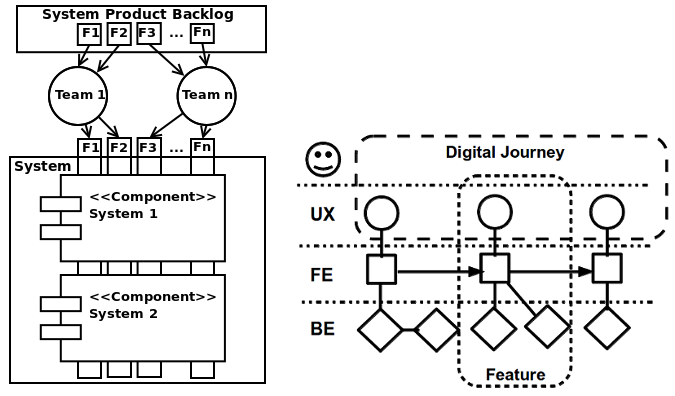
\includegraphics[width=0.80\textwidth]{ScrumTeamsByFeatures}
  \caption{Esquema de equipos de características}
  \centering
  \label{fig:ScrumTeamsByFeatures} %\ref{fig:ScrumTeamsByFeatures}
\end{figure}

En esta arquitectura de organización es necesario coordinar el trabajo de los diferentes equipos. Los Scrum Master deben reunirse con regularidad, promoviendo la transformación a través de una lista visible de los impedimentos de organización. Los Scrum Master, además deberán estar familiarizados con biografía relacionada a este problema de escalabilidad como "Scaling Lean and Agile Development" \cite{Larman-Vodde-2008}.

\subsection{Equipos de componentes}

Abordar el problema de proyectos grandes con "Equipos Scrum de componentes" (ver figura \ref{fig:ScrumTeamsByComponent}) consiste en que cada equipo sólo es responsable de la ejecución de ciertos componentes dedicados en el sistema de los cuales el equipo es dueño de su desarrollo. Desde esta perspectiva se pueden tener equipos dedicados por capas (capa front-end, capa de servicios, capa de persistencia) y por componentes de arquitectura de software (diferentes componentes como librerías, servicios o subsistemas).

\begin{figure}[h]
  \centering
  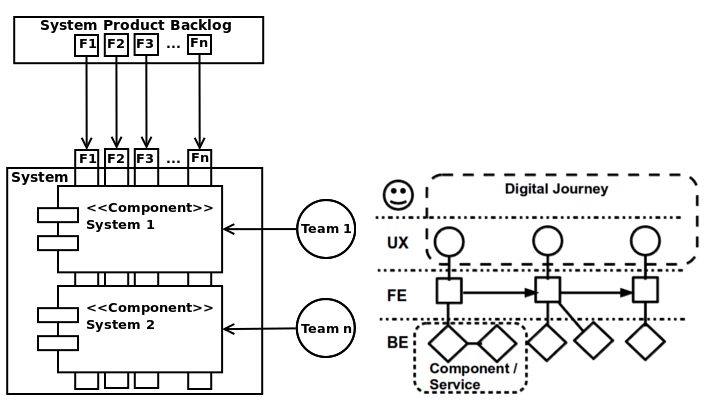
\includegraphics[width=0.80\textwidth]{ScrumTeamsByComponent}
  \caption{Esquema de equipos de componentes}
  \centering
  \label{fig:ScrumTeamsByComponent} %\ref{fig:ScrumTeamsByComponent}
\end{figure}

Para terminar una PBI o historia de usuario hay en la mayoría de los casos la necesidad de dividir las historias en partes más pequeñas que podrían ser implementadas dentro de un solo componente. Además se genera dependencias entre los diferentes equipos haciendo necesario procesos de integración periódica y coordinación de equipos. En muchos casos, una sola historia de usuario no se puede implementar dentro de un único sprint y, en su defecto, depende de los resultados de otras historias desarrolladas por otro equipo que aún no están disponibles. A esto se lo llama "pipeline" y debe evitarse en lo posible o gestionarse apropiadamente.

La ventaja de utilizar equipos de componentes es que es más fácil asegurar una determinada arquitectura del sistema. Por ejemplo si se quiere asegurar una Arquitectura SOA o una de Microservicios que está orientada a componentes. Esta idea está, entre otras cosas, basada en la "Ley de Conway"\footnote{Conway's Law \cite{Conway-1968} no es exactamente una ley, sino que es más bien una observación que Conway publicó en 1968.} que sugiere que las organizaciones pueden replicar su arquitectura en los productos que ellas producen \cite{Martin-Fowler-2014}. 

Por otro lado, puede tener como desventaja que las personas se pueden especializar sólo en pequeñas partes del sistema y el conocimiento global sobre el sistema en su conjunto podría perderse \cite{Scrum-Institute-2015}. En este caso podría tener lugar una optimización local, ya que el equipo a veces puede tomar decisiones que están optimizadas para el componente individual, pero las mejores soluciones desde una perspectiva del sistema total podrían haber sido desestimadas u obviadas.


\subsection{Equipos mixtos}

También es posible la configuración de equipos mixtos que son la combinación de equipos de características y de componentes (ver figura \ref{fig:ScrumTeamsMix}).

\begin{figure}[h]
  \centering
  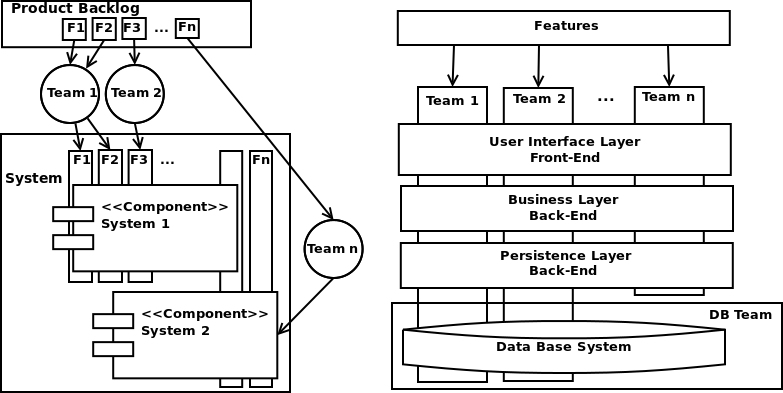
\includegraphics[width=0.99\textwidth]{ScrumTeamsMix}
  \caption{Ejemplo de equipos mixtos.}
  \centering
  \label{fig:ScrumTeamsMix} %\ref{fig:ScrumTeamsMix}
\end{figure}

\section{Integración}

\subsection{Scrum de Scrum}

Scrum de Scrum es una forma de organización y técnica para escalar Scrum a grupos grandes de personas u organizaciones con proyectos grandes, programas o portfolios. Consiste en distinguir un integrante con el rol de Embajador, denominado "Ambassador", por cada Equipo Scrum \cite{Stefanini-2013}. El Embajador será quien participará en reuniones Daily con Embajadores de otros equipos. A esta reunión de Embajadores se la llama "Scrum de Scrum" o SoS. Habitualmente se usa que el rol de Embajador lo desempeñe el Scrum Master, pero puede ser desempeñado por otro integrante del Equipo de Desarrollo. También puede ser desempeñado por un integrante del Equipo acompañado del Scrum Master.

La reunión SoS se comporta como una Daily donde los Embajadores reportan la situación de su equipo y sus impedimentos. El embajador de cada equipo comenta la respuesta a las siguientes tres preguntas:

\begin{itemize}
\item \textbf{¿Qué hicimos ayer?}
\item \textbf{¿Qué vamos a hacer hoy?}
\item \textbf{Si tenemos obstáculos: ¿Qué impedimentos tenemos?} ¿Qué impedimentos tenemos a nivel de equipo? ¿Si algún otro equipo nos bloquea para algo? ¿Si bloqueamos en algo a algún otro equipo?
\end{itemize}

La SoS puede ser facilitada y moderada por una persona que puede desempeñar un rol de facilitador, coordinador e integrador inter-equipos. Este rol puede tener diferentes nombres y el SBOK lo denomina Chief Scrum Master o CSM. El CSM apoyará y brindará soporte a los SM de diferentes equipos.

\subsection{Scrum de Scrum de Scrum}

En organizaciones donde hay muchos Equipo Scrums trabajando en varias partes de un proyecto o producto grande, puede ser necesario otro nivel más de coordinación, ya que hay equipos que no participan en SoS de otras áreas. Aquí es cuando se aplica la "Scrum of Scrum of Scrum"\footnote{\cite{SBOK-2013}} o SoSoS, que consiste en una reunión frecuente a un nivel superior de la SoS.

\subsection{Comunidades}

En una organización grande, independientemente de Scrum, se suelen formar comunidades. Estas comunidades se dan por especialidades técnicas o roles. Las mismas son útiles para colaboración entre equipos, generación de discusiones globales y resolución de problemas transversales. Es aconsejable que se den en forma orgánica. Aunque son particularmente útiles las comunidades de SM y de PO. La de SM es una posibilidad de mejora contínua del marco de trabajo y la de PO puede funcionar como equipos de PO para tratar temas del negocio transversal y administrar backlog en conjunto.

\begin{figure}[h]
  \centering
  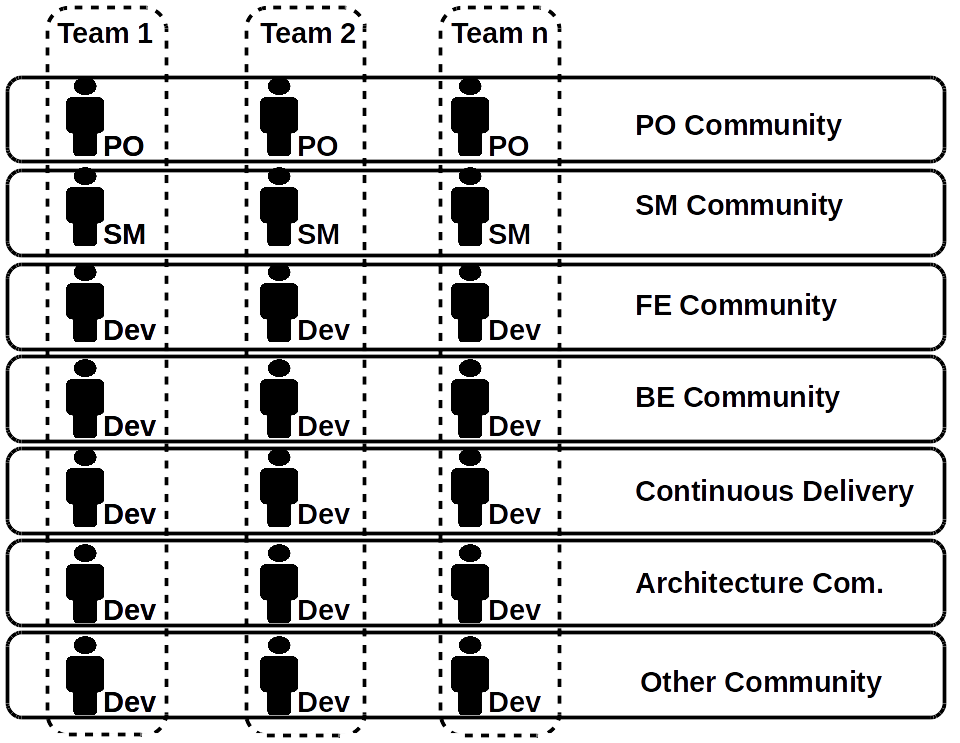
\includegraphics[width=0.60\textwidth]{Communities}
  \caption{Ejemplo de comunidades}
  \centering
  \label{fig:Communities} %\ref{fig:Communities}
\end{figure}


\subsection{Integración UX}

Un desafío a la hora de hacer Scrum es incorporar UX en el desarrollo incremental por sprints. Se pueden adoptar, entre otras, dos estrategias principales: desarrollo UX distribuido y gobernado; o desarrollo UX centralizado (equipo externo).

\subsubsection{Desarrollo UX Distribuido y Gobernado}

Una estrategia es tener UXer, como miembros de equipo Scrum, distribuidos en cada equipo. Esto permite empoderamiento y velocidad, pero puede generar una UX poco unificada o con poca “integridad conceptual”. Para resolver este problema de unificación se puede acudir a la estandarización UX. La misma podría ser generada y mantenida por los equipos o mediante un equipo externo responsabilizado de la integridad conceptual y experiencia unificada (equipo de estandarización UX transversal) y usar un sistema de versionado de estándares que sirve como otra herramienta de coordinación.

\subsubsection{Desarrollo UX Centralizado}

Otra estrategia es tener un equipo externo de UX que agrupe a todos los UXer y que provea, como un equipo de servicios, los diseños UX a los equipos de desarrollo. Sin embargo, es probable que el equipo central se convierta en un “cuello de botella” para los equipos de desarrollo y, además, pueda generar más “dependencias” que deben ser abordadas. Para mitigar estos problemas, un modelo híbrido a menudo puede ser aplicado, además de mecanismos de coordinación entre el equipo central y los equipos restantes.

\subsubsection{Mecanismo de coordinación de tarea UX en una historia}

En ambas propuestas es necesario coordinar e integrar el flujo de trabajo UX con el flujo de desarrollo Scrum. Esto sucede principalmente porque el flujo de trabajo UX no suele entrar dentro de un sprint corto (dos semanas) para que las historias puedan ser finalizadas. Lo que se puede hacer, es que el trabajo UX sea previo al sprint (adelantado al sprint) como parte de la etapa de refinamiento, o como etapa previa al compromiso de planning de sprint. La historia no se termina de refinar o no se compromete en un sprint, hasta que no se considera el trabajo UX lo suficientemente maduro como para que sea abordada para desarrollo. Una manera de hacer esta sincronización es agregando una cláusula de completitud de tarea UX al DoR de la historia. Y, además, asociando a las historias tareas UX que, a su vez, tengan DoR y DoD propios. De este modo, una tarea UX no se considera terminada, para que su historia asociada sea abordada en un sprint, si no cumple su “DoD UX”. Además, para trabajar a sprint adelantado hay que considerara que antes del sprint 1 debería hacerse un sprint 0 (sprint metáfora y/o inception).

\begin{figure}[h]
  \centering
  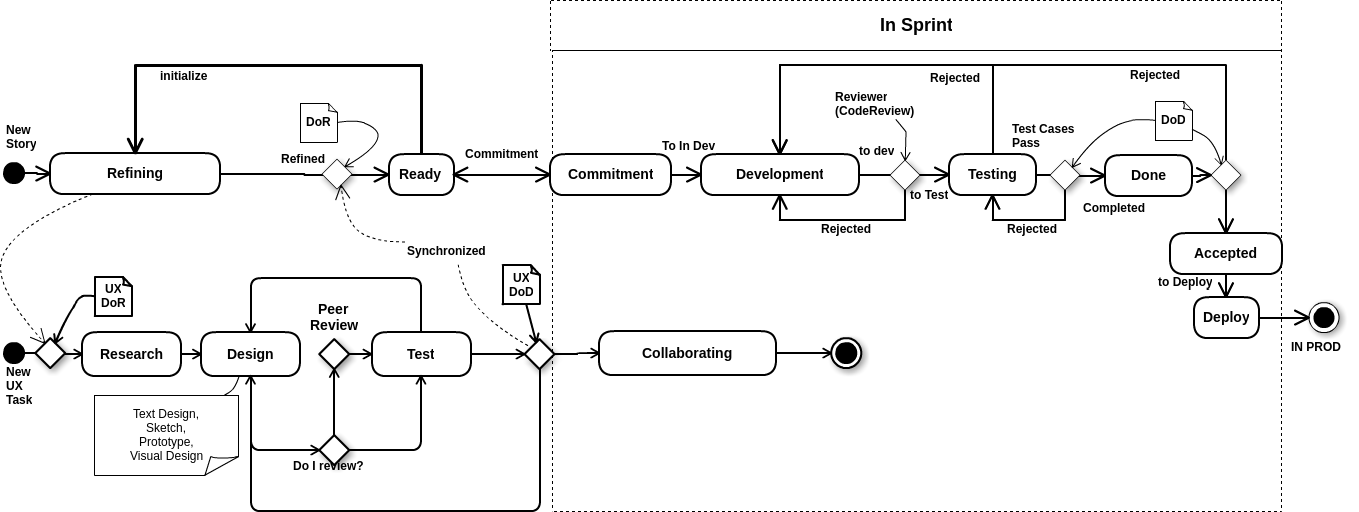
\includegraphics[width=1\textwidth]{UXtask-and-Story-in-Scrum}
  \caption{Ejemplo de coordinación entre flujos de tarea UX e historia}
  \centering
  \label{fig:UXtask-and-Story-in-Scrum} %\ref{fig:UXtask-and-Story-in-Scrum}
\end{figure}

\subsection{DevOps}

La integración a escala para que una Software Factory sea ágil y lleve adelante uno de sus principios, el Continuous Delivery, es lo que se denomina DevOps. DevOps es la integración de Ingeniería de Desarrollo de Software con la Ingeniería de Operaciones, que es todo el soporte IT y de plataforma para posibilitar que el proceso de desarrollo sea ágil, haciendo entregas frecuentes de calidad y logrando la colaboración entre el personal de desarrollo y el personal de operaciones a lo largo de todas las etapas del ciclo de vida de producción de software. DevOps es una parte central del agilismo en la entrega de software eficiente, por medio de la integración de equipos, metodologías ágiles, técnicas y stack tecnológico como una sola organización. El objetivo principal de DevOps es minimizar los cuellos de botella en el pipeline de entrega, haciéndolo más eficiente y ágil \footnote{\cite{DevOps-for-dummies-2015}}.

\begin{figure}[h]
  \centering
  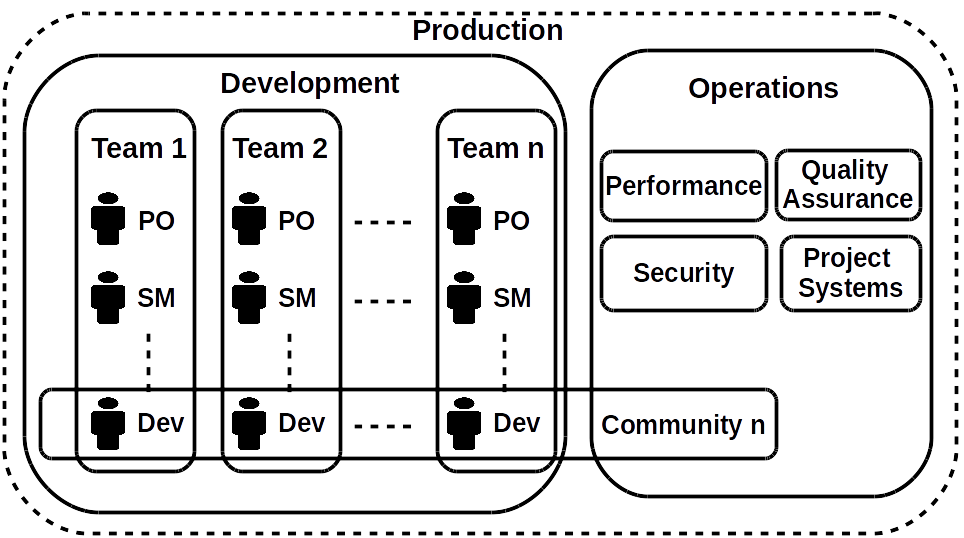
\includegraphics[width=0.80\textwidth]{DevOps}
  \caption{Ejemplo de integración de equpos en DevOps}
  \centering
  \label{fig:DevOps} %\ref{fig:DevOps}
\end{figure}

Una manera de integrar Operaciones con Desarrollo es mediante el uso de herramientas compartidas, misma cultura, comunidades en común, procesos ágiles compartidos, comunicación estandarizada, etcétera. Algo crucial en una organización madura es la automatización máxima en procesos de Continuous Integration y Continuous Delivery.

En cuanto a Scrum, el área de operaciones no necesita implementar Scrum, pero sí puede llevar en práctica sus valores, ser ágil (con Lean, Kanban, DAD, etc.) y tener en cuenta los ciclos Scrum de los equipos de desarrollo. DevOps es sólo un paso importante para unirse a la cultura general de la colaboración ágil y que debe involucrar a todas las disciplinas en una organización. 


\section{Modelos de escalamiento}

Existen diversos modelos, marcos y frameworks para escalamiento como lo son el modelo Spotify, SAFe, LeSS, Nexus, DAD, Lean Management, Agile Portfolio Management (APM), Recipes for Agile Governance in the Enterprise (RAGE) y otros. A continuación una breve reseña de algunos de ellos.

\subsection{Spotify}

Spotify es un caso de estudio que demuestra que puede ser aplicado más allá de pequeñas empresas o startup, sino en empresas más grandes (Spotify constaba en 2014 de aproximadamente de 250 personas en tres países). Por este motivo es un modelo de referencia. El modelo de Spotify consta de equipos escuadrones (squad), equivalentes a Equipos Scrum, con un PO y un SM llamado también Team Facilitator (Coach del equipo). Los escuadrones relacionados se agrupan en tribus (tribe) de no más de 100 personas, conformando un área de producto (como por ejemplo un tipo de producto) o área funcional (como por ejemplo infraestructura). La tribu tiene un líder de tribu (Tribe lead) quien se encarga de asegurar un alto rendimiento de la tribu, dar soporte a los líderes de los capítulos, facilitar y entrenar a los SM y construir liderazgo dentro de la tribu. 

\begin{figure}[h]
  \centering
  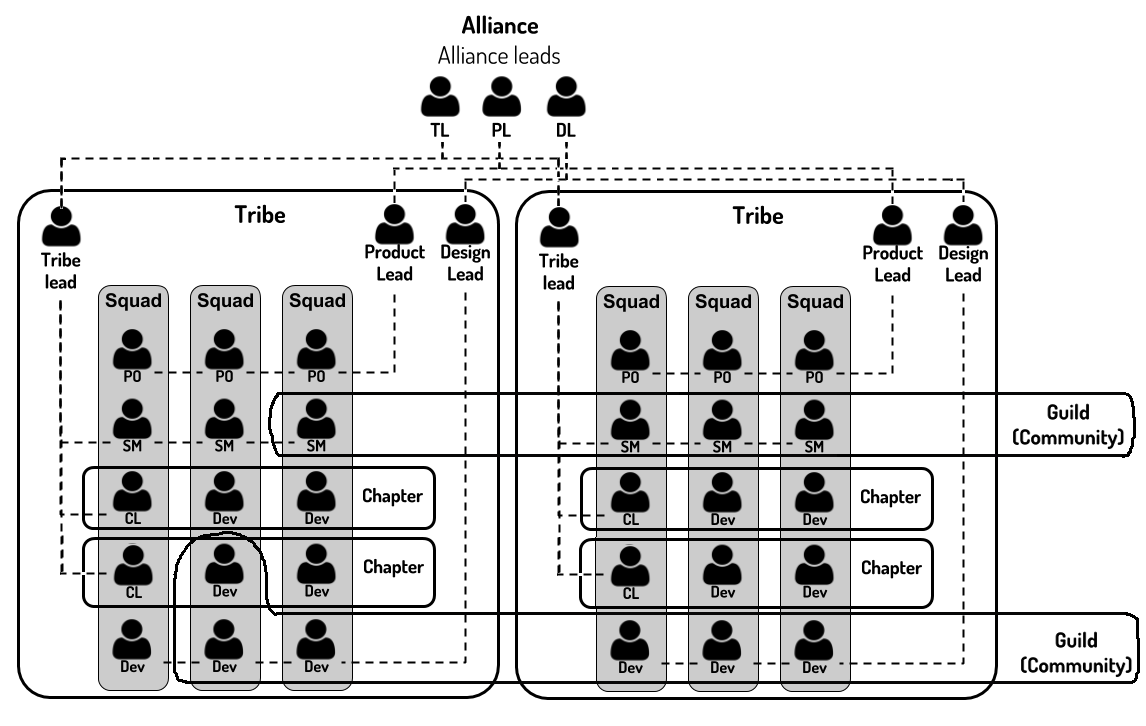
\includegraphics[width=0.99\textwidth]{Spotify_organizational_model}
  \caption{Modelo organizacional Spotify}
  \centering
  \label{fig:Spotify_organizational_model} %\ref{fig:Spotify_organizational_model}
\end{figure}

La tribu también tiene un líder de producto (PL) y uno de diseño (DL). Dentro de cada tribu hay capítulos (Chapter) y cada uno engloba un área funcional técnica de ingeniería, agrupando a los miembros de diferentes escuadrones con habilidades similares y que trabajan dentro del mismo área de competencia (por ejemplo el capítulo QA, BE, FE, etc.). Cada capítulo tiene un líder del capítulo ("Chapter lead" o CL) quien se encarga del desarrollo profesional, la cultura de la ingeniería, el apoyo del escuadrón y en asegurar la contratación de las personas adecuadas. Los líderes de capítulo suelen ser desarrolladores a tiempo parcial, por lo general se sientan en uno de los escuadrones de la tribu. 
Las diferentes tribus se pueden relacionar de diferentes maneras. Dos de ellas son la alianza (Alliance) y las comunidades (Guild). Una comunidad es una "comunidad de interés" (explicadas anteriormente). Los capítulos siempre son locales para una tribu, mientras que una comunidad generalmente es transversal a varias tribus. Cada comunidad puede tener un "coordinador de comunidad" y su alcance es más flexible. Y por último, la alianza une a diferentes comunidades por cohesión funcional de producto y tiene tres líderes serviciales (TL, PL y DL) quienes facilitan el trabajo de los líderes de las tribus unidas y el funcionamiento de las tribus, en general.

\subsection{SAFe}

El framework Scaled Agile Framework o SAFe consiste en una base de conocimientos de patrones integrados modulares, por niveles organizativos, destinados al desarrollo Lean-Agile a escala empresarial. Scrum se integra en SAFe en el primer nivel inferior organizativo, el nivel de equipo. A este nivel le siguen los niveles de programa, flujo de valor y portafolio. SAFe propone elementos opcionales de integración, un nuevo rol llamado Product Manager quien dirige a los POs de los equipos, otro nuevo rol llamado Release Train Engineer quien coordina a los SMs, la coordinación de backlogs por medio de un Backlog a nivel programa y la coordinación entre equipos por medio de eventos conjuntos y refinamientos, eventos trimestrales, System Team, Scrum of Scrums, Team Backlog y Team PO. SAFe propone que los equipos deben tener sus iteraciones sincronizadas y a tiempos periódicos deben tener una iteración de integración y planificación de todos los equipos o productos  (se planifican trenes de releases). Para más información hay que remitirse a la guía y definición de prácticas dada por el sitio web de SAFe.

\subsection{LeSS}

Por otro lado tenemos al framework Large-Scale Scrum o LeSS que  es un marco de desarrollo de productos que extiende Scrum con reglas de escalado y directrices sin perder los propósitos originales de Scrum. LeSS tiene un conjunto de principios alineados a Scrum y sumado el pensamiento sistémico. Además tiene alrededor de 28 reglas disponibles en 3 libros y propone diferentes mecanismos de coordinación como eventos conjuntos y refinamiento, CoP, SoS, Integración de código, feature teams y Area Product Owner. LeSS también propone subdivisiones de la organización por áreas de valor o Customer Value. Para más información hay que buscar en la guía del sitio web “less.works” y en diferentes libros que tratan el tema, como por ejemplo: Large-Scale Scrum, More with LeSS de Craig Larman y Bas Vodde.

\subsection{Modelo Nexus}

Nexus es un marco de trabajo para desarrollar y mantener iniciativas a escala de desarrollo de productos y software basado en Scrum. Fue creado por Ken Schwaber y Scrum.org. Es un exoesqueleto cuyo corazón es un conjunto de Equipos Scrum combinados para crear un Incremento Integrado, usando una única Lista de Producto Backlog, manteniendo "Listas de Pendientes" por Sprint y apoyados por un "Equipo de Integración Nexus" quien brinda soporte para asegurar que se produzca un Incremento Integrado. Para más información basta leer la "Guía Nexus" publicada en Scrum.org.

\subsection{DAD}

El marco de decisiones de procesos “Disciplined Agile Delivery” o DAD, brinda una orientación ligera para ayudar a las organizaciones a escalar agilidad y buscar optimizar sus procesos de tecnología de la información (IT) de una manera sensible al contexto ágil y DevOps. Para ello, muestra cómo las diversas actividades, como la entrega de soluciones, las operaciones, la arquitectura empresarial, la gestión de cartera y otros equipos y áreas trabajan juntas. Las reglas implicadas en este marco hacen que la empresa busque ser consciente y escalable. La referencia primaria para DAD es el libro “Disciplined Agile Delivery: A Practitioner's Guide to Agile Software Delivery in the Enterprise”,  escrito por Scott Ambler y Mark Lines.\newline
\newline

Si bien estos modelos tiene distintos grados de aceptación y éxito en muchas organizaciones, no se deben tomar como ley en piedra aplicándolos en cualquier contexto u organización. No se deberían implementar como recetas a seguir o soluciones ideales a implantar. Para aplicarlos en una organización deben ser evaluados y, en caso de aplicar alguna de sus pautas, ajustados según contexto y necesidades. Se recomienda aplicar también el pensamiento sistémico, ingeniería de sistemas y perspectivas de otras disciplinas.

\section{Equipo de mejora continua}

Como se ha visto, el escalamiento no es tarea simple y no existe una solución universal. Se puede dejar que los cambios organizacionales emerjan de abajo hacia arriba (desde los equipos, comunidades o individuos), sean dirigidos por un ente director (coaches, consultoras o un líder transformacional) o algo mixto. Hay frameworks que recomiendan que, cuando se desea llevar a cabo transformaciones organizacionales hacia la agilidad, se constituya un equipo de expertos ágiles llamado centro de excelencia, centro de transformación digital, centro de soporte ágil o equipo transversal de mejora continua \footnote{ScrumStudy recomienda un Scrum Guidance Body y DAD recominda un equipo de excelencia CoE.}. Este equipo se encargaría de hacer coaching a equipos y a otros roles, proponer iniciativas de mejoras organizacionales y apoyar la transformación cultural. El equipo puede estar formado por Coaches Ágiles Empresariales, gerentes ágiles, ingenieros de sistemas, ingenieros de operaciones, capital humano, etc. Los miembros deben ser capaces de trabajar en cualquier nivel de la organización, teniendo una visión multidisciplinaria, global y perspectiva sistémica.

\chapter{Glosario y Acrónimos}

\begin{table}[h]
\begin{tabular}{lllll}
\cline{1-2}
\multicolumn{1}{|l|}{Nombre}   & \multicolumn{1}{l|}{Descripción}  &  &  &  \\ \cline{1-2}
\multicolumn{1}{|l|}{Artifact}   & \multicolumn{1}{l|}{Artefacto o almacén de incisos de trabajo}  &  &  &  \\ \cline{1-2}
\multicolumn{1}{|l|}{BDUF}   & \multicolumn{1}{l|}{Gran diseño al inicio (Big Design Up Front)}  &  &  &  \\ \cline{1-2}
\multicolumn{1}{|l|}{DoD}   & \multicolumn{1}{l|}{Definición de terminado (Definition of Done)}  &  &  &  \\ \cline{1-2}
\multicolumn{1}{|l|}{DoR}   & \multicolumn{1}{l|}{Definición de completitud (Definition of ready)}  &  &  &  \\ \cline{1-2}
\multicolumn{1}{|l|}{DT}   & \multicolumn{1}{l|}{Equipo de desarrollo (Development Team)}  &  &  &  \\ \cline{1-2}
\multicolumn{1}{|l|}{DUF}   & \multicolumn{1}{l|}{Diseño al inicio (Design Up Front)}  &  &  &  \\ \cline{1-2}
\multicolumn{1}{|l|}{Features}   & \multicolumn{1}{l|}{
\begin{tabular}[c]{@{}l@{}}
Representan interacciones y acciones del usuario con\\ 
el sistema. \\ 
Son funcionalidades que entregan valor de cara al usuario.\\
\end{tabular}
}  &  &  &  \\ \cline{1-2}
\multicolumn{1}{|l|}{MMP}   & \multicolumn{1}{l|}{(Minimal Marketable Product) Producto comerciable mínimo.}  &  &  &  \\ \cline{1-2}
\multicolumn{1}{|l|}{MVP}   & \multicolumn{1}{l|}{(Minimal Viable Product) Producto viable mínimo.}  &  &  &  \\ \cline{1-2}
\multicolumn{1}{|l|}{PB}   & \multicolumn{1}{l|}{Backlog de producto (Product Backlog)}  &  &  &  \\ \cline{1-2}
\multicolumn{1}{|l|}{PBI}   & \multicolumn{1}{l|}{Ítem de PB (Product Backlog Item)}  &  &  &  \\ \cline{1-2}
\multicolumn{1}{|l|}{PI}   & \multicolumn{1}{l|}{Incremento de producto (Product Increment)}  &  &  &  \\ \cline{1-2}
\multicolumn{1}{|l|}{PMI}   & \multicolumn{1}{l|}{
\begin{tabular}[c]{@{}l@{}}
Instituto de Gestión de Proyectos \\
(Project Management Institute) \\
\end{tabular}
}  &  &  &  \\ \cline{1-2}
\multicolumn{1}{|l|}{PO}   & \multicolumn{1}{l|}{Dueño del producto (Product Owner)}  &  &  &  \\ \cline{1-2}
\multicolumn{1}{|l|}{ROI}   & \multicolumn{1}{l|}{Retorno de la inversión (Return On Investment)}  &  &  &  \\ \cline{1-2}
\multicolumn{1}{|l|}{SCRUM}   & \multicolumn{1}{l|}{
\begin{tabular}[c]{@{}l@{}}
Es un juego de rugby en el que, por lo general, tres\\
miembros de cada línea se unen opuestos unos a \\
otros con un grupo de dos y un grupo de tres \\
jugadores detrás de ellos, lo que hace un grupo \\
de ocho personas, tres, dos, tres formados en cada \\
lado; el balón se deja entre la línea divisoria de \\
ambos grupos, los jugadores están abrazados \\
y tomados de la cintura de un compañero de equipo\\
y los del frente hombro a hombro con el oponente,\\
y se trata hacer fuerza grupalmente para desplazar \\
al grupo rival y patear la pelota hacia atrás para \\ 
que un compañero de equipo la tome.\\
\end{tabular}
}  &  &  &  \\ \cline{1-2}
\multicolumn{1}{|l|}{SB}   & \multicolumn{1}{l|}{Backlog de iteración (Sprint Backlog)}  &  &  &  \\ \cline{1-2}
\multicolumn{1}{|l|}{SM}   & \multicolumn{1}{l|}{Facilitador (ScrumMaster)}  &  &  &  \\ \cline{1-2}
\multicolumn{1}{|l|}{SOA}   & \multicolumn{1}{l|}{
\begin{tabular}[c]{@{}l@{}}
Arquitectura Orientada a Servicios \\
(Service-Oriented Architecture) \\
\end{tabular}
}  &  &  &  \\ \cline{1-2}
\multicolumn{1}{|l|}{SP}   & \multicolumn{1}{l|}{Iteración (Sprint)}  &  &  &  \\ \cline{1-2}

%% Ejemplo de como agregar una fila con saltos de linea
%% \multicolumn{1}{|l|}{Example}   & \multicolumn{1}{l|}{
%% \begin{tabular}[c]{@{}l@{}}
%% texto texto texto texto texto texto texto  \\
%% texto texto texto texto texto texto texto \\
%% \end{tabular}
%% }  &  &  &  \\ \cline{1-2}

                           &                                                          &  &  & 
\end{tabular}
\end{table}


% Bibliography
\bibliographystyle{apalike}
\bibliography{content/bibliography_list}

\end{document}
